\documentclass{article}
\usepackage{amsmath}
\usepackage{amsfonts}
\usepackage{graphicx}
\usepackage{geometry}
\usepackage{bm}
\geometry{top=2.5cm,left=2.5cm,right=2.5cm,bottom=2.5cm}
\title{Numeric Simulation}
\author{}
\date{}
\begin{document}
\maketitle
In this section results of some numeric simulation experiments are reported. We tested our algorithm on the following four models:
\begin{itemize}
	\item 4-dimension sphere $\mathbb{S}^4$ embedded in 5 dimension Eulidean space.
	\item 3-dimension flat torus $\mathbb{T}^3$ embedded in 4 dimension Euclidean space.
	\item 2-dimension curved torus embedded in 3 dimension space
	\item 2-dimension pseudosphere embedded in 2 dimension space
\end{itemize}
For every model, we fixed the sample size 20000, and sampled uniformly distributed on it (specified later). Then we choose epsilon such that for each point the average number of neighbors is approximately $10^2$. We randomly choose one point a time in every model, calculate the Riemann curvature there as we proposed and then repeat the whole process for 10000 times. The results are evaluated (specified later) basically by the mean absolute value of the Frobenius norm of our estimated $\widehat{\boldsymbol{R}}$ and the true value $\boldsymbol{R}$
\\
\par
\textbf{4d-Sphere in $\mathbb{R}^5$} The data is sampled as \cite{Uniform}, we generate 4-dimension standard normal distribution random numbers and then normalise them to get uniform distributed data. The true value of Riemann curvature tensor of a 4d-sphere with radius $R$ is
\begin{equation}
	R_{ijkl}=\frac{1}{R^2}(g_{il}g_{jk}-g_{ik}g_{jl})
\end{equation}
for any basis. Therefore with $R=1$,the true value of $\boldsymbol{R}$ is
\begin{equation}
	\boldsymbol{R}=(\overbrace{-1,-1,\cdots,-1}^{6},\overbrace{0,0,\cdots,0}^{10})
\end{equation} In case that the average number of neighbors for every point is approximately 100, we choose $\epsilon=0.40$
Then the distribution of repeated result of estimation can be shown in figures. 
\begin{figure}[htbp]
\centering
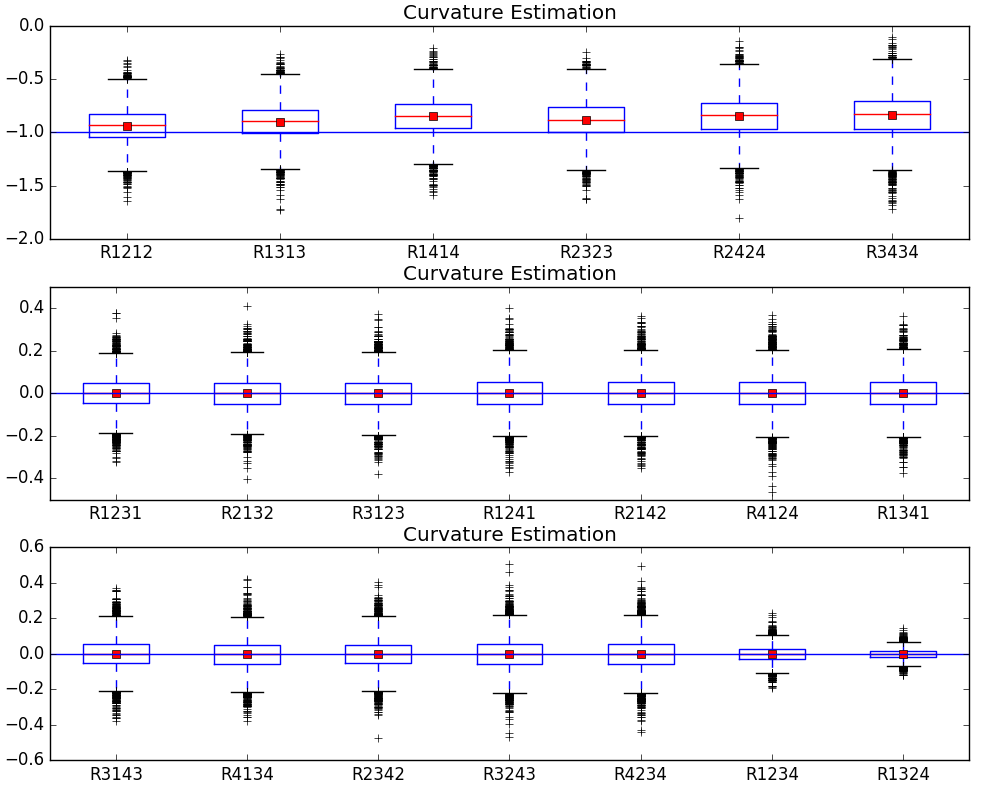
\includegraphics[width=0.8\textwidth]{sphere4d.png}
\end{figure}

\par
\textbf{3d-Flat torus in $\mathbb{R}^4$} Here the 3d-flat torus is given by the parametrization
\begin{equation}
	(\cos u,\sin u,\cos v,\sin v, \cos w,\sin w),\quad u,v,w\in[0,2\pi)
\end{equation}
And the true value for every component is 0 according to standard calculation of Riemann curvature tensor. The data is sampled uniformly by first finding uniformly distributed sample on three perpendicular $\mathbb{S}^1$ circles and then generate there cartesian product.In our simulation, we select $R=2,r=1$. We choose epsilon = $0.63$ to guarantee approximately 100 neighbors in average for every point. The true value of curvature tensor for flat torus is zero for every component. The estimation results are shown in figures.
\begin{figure}[htbp]
\centering
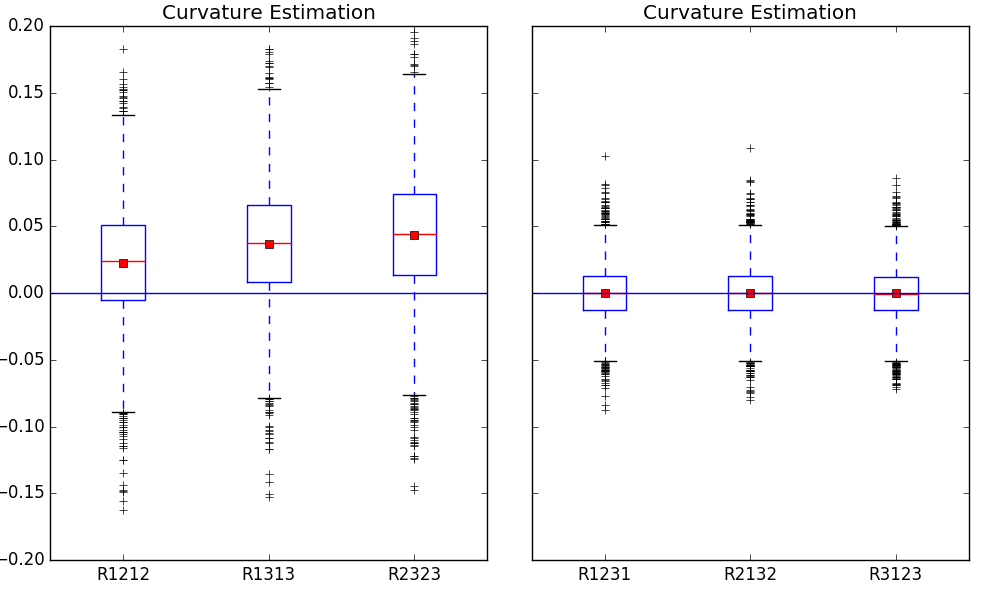
\includegraphics[width=0.8\textwidth]{torus.png}
\end{figure}
\\
\par
\textbf{2d-curved torus in $\mathbb{R}^3$} Here we test our algorithm on varying sectional curvature case. The curved torus is given by the parametrization
\begin{equation}
	((R+r\cos \theta)\cos\phi, (R+r\cos \theta)\sin\phi,r\sin\theta),\quad 0\leq \theta,\phi \leq 2\pi
\end{equation}
Sampling is conducted as \cite{Sample} Example 1A. At point $(\theta,\phi)$, since it is only two dimensional, the only one independent component of the curvature tensor is $R_{1212}=-\frac{\cos \theta}{R+r\cos \theta}$. Then we can see the estimated result as
\begin{figure}[htbp]
\centering
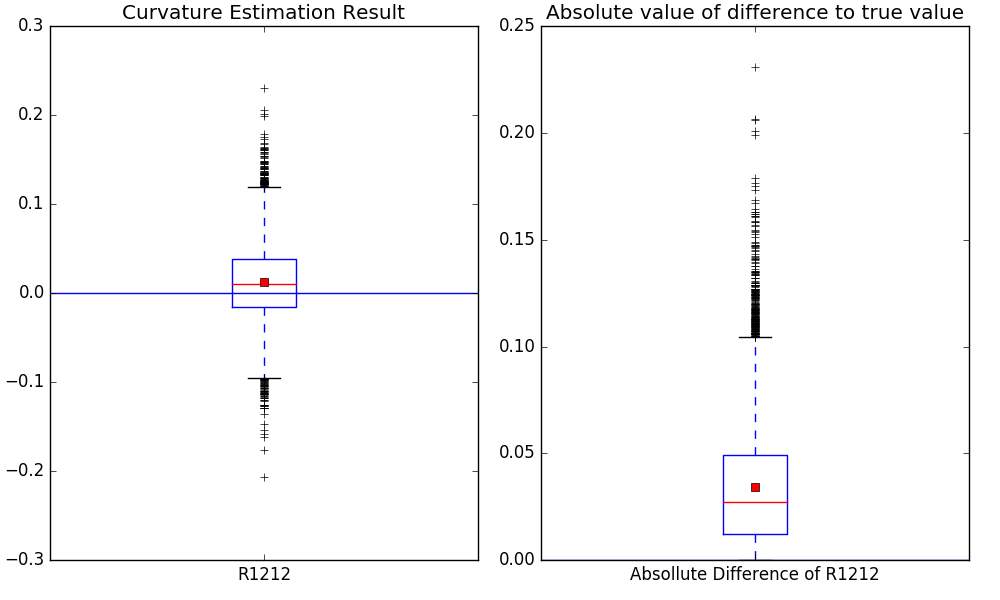
\includegraphics[width=0.8\textwidth]{ctorus.png}
\end{figure}

\par
\textbf{2d-pseudosphere in $\mathbb{R}^3$} Pseusosphere is one representative of negative constant gaussian curvature, given by the parametrization
\begin{equation}
	(\cos u \sin v, \sin u\sin v, \cos u+\log(\tan(\frac{v}{2}))),\quad u\in[0,2\pi), v\in [0,\pi)
\end{equation}
We choose $\epsilon = 0.2$ to have a proper number of average neighbors. The results are shown as
\begin{figure}[htbp]
\centering
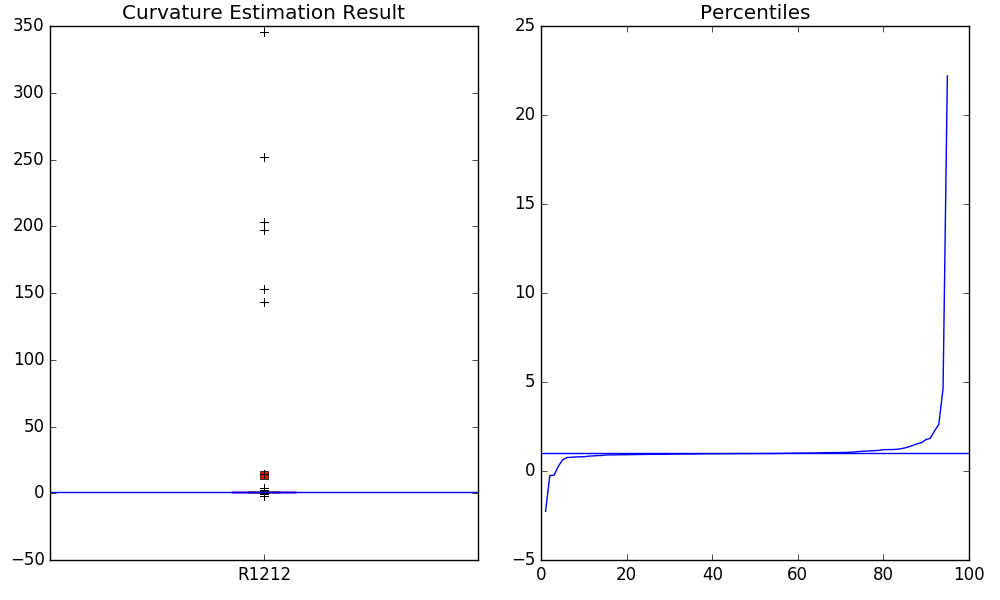
\includegraphics[width=0.8\textwidth]{psphere.png}
\end{figure}
\bibliography{curve}
\bibliographystyle{plain}

\end{document}